\newpage

\changeindent{0cm}
\section{実験}
\changeindent{2cm}

%%%%%%%%%%%%%%%%%%%%%%%%%%%%%%
%\afterpage{\clearpage}
\subsection{実験 1}

文章の話題ごとに皮肉か非皮肉かを推定する実験に取り組んだ.
モデルには BERT を使用し,データセットには SARC 2.0 main balanced データセットを使用した.
\par
まず subreddit ごとにデータを抽出し,新たにデータセットを作成した.
その際にテストデータが 1,500 件以上取得できたものを選択し,politics,AskReddit,worldnews,pcmasterrace の 4 つのデータセットを実験に使用した.
また比較のため,全ての subreddit からランダムにデータをサンプリングした random データセットを作成し実験に使用した.
このとき同じ親投稿を持つ皮肉データと非皮肉データのペアは崩さないように抽出した.
random データセットに含まれる subreddit を確認したところ,訓練データは 1,257 種類,テストデータは 569 種類の subreddit から構成されていた.
表 \ref{tb:4_subreddit_data} に各データセットのデータ数を示す.
なお各データセットには皮肉データと非皮肉データは同数含まれている.

%%% table
\begin{table}[b]
  \caption{各データセットのデータ数}
  \label{tb:4_subreddit_data}
  \centering
  \begin{tabular}{c c c} \hline

データセット & 訓練 (件) & テスト (件) \\ \hline
politics & 13,668 & 3,406 \\
AskReddit & 11,660 & 3,006 \\
worldnews & 9,444 & 2,246 \\
pcmasterrace & 7,400 & 1,772 \\
random & 14,000 & 3,500 \\ \hline

  \end{tabular}
\end{table}
% end

\par
図 \ref{fig:40_model} にモデルの概要を示す.
まず入力の先頭に [CLS] トークンを,各コメントの末尾に [SEP] トークンを付けて BERT に入力し,分散表現を取得した.
分散表現のうち,文頭の [CLS] トークンに該当する分散表現を入力文章全体の分散表現とみなし,それを線形層に入力して皮肉か非皮肉かを二値分類した.
訓練データでモデルを学習し,テストデータでその性能を評価した.
評価指標には Accuracy(正解率),Precision(適合率),Recall(再現率),F1 値を使用した.

% figure model
 \begin{figure}[tb]
 	\begin{center}
	 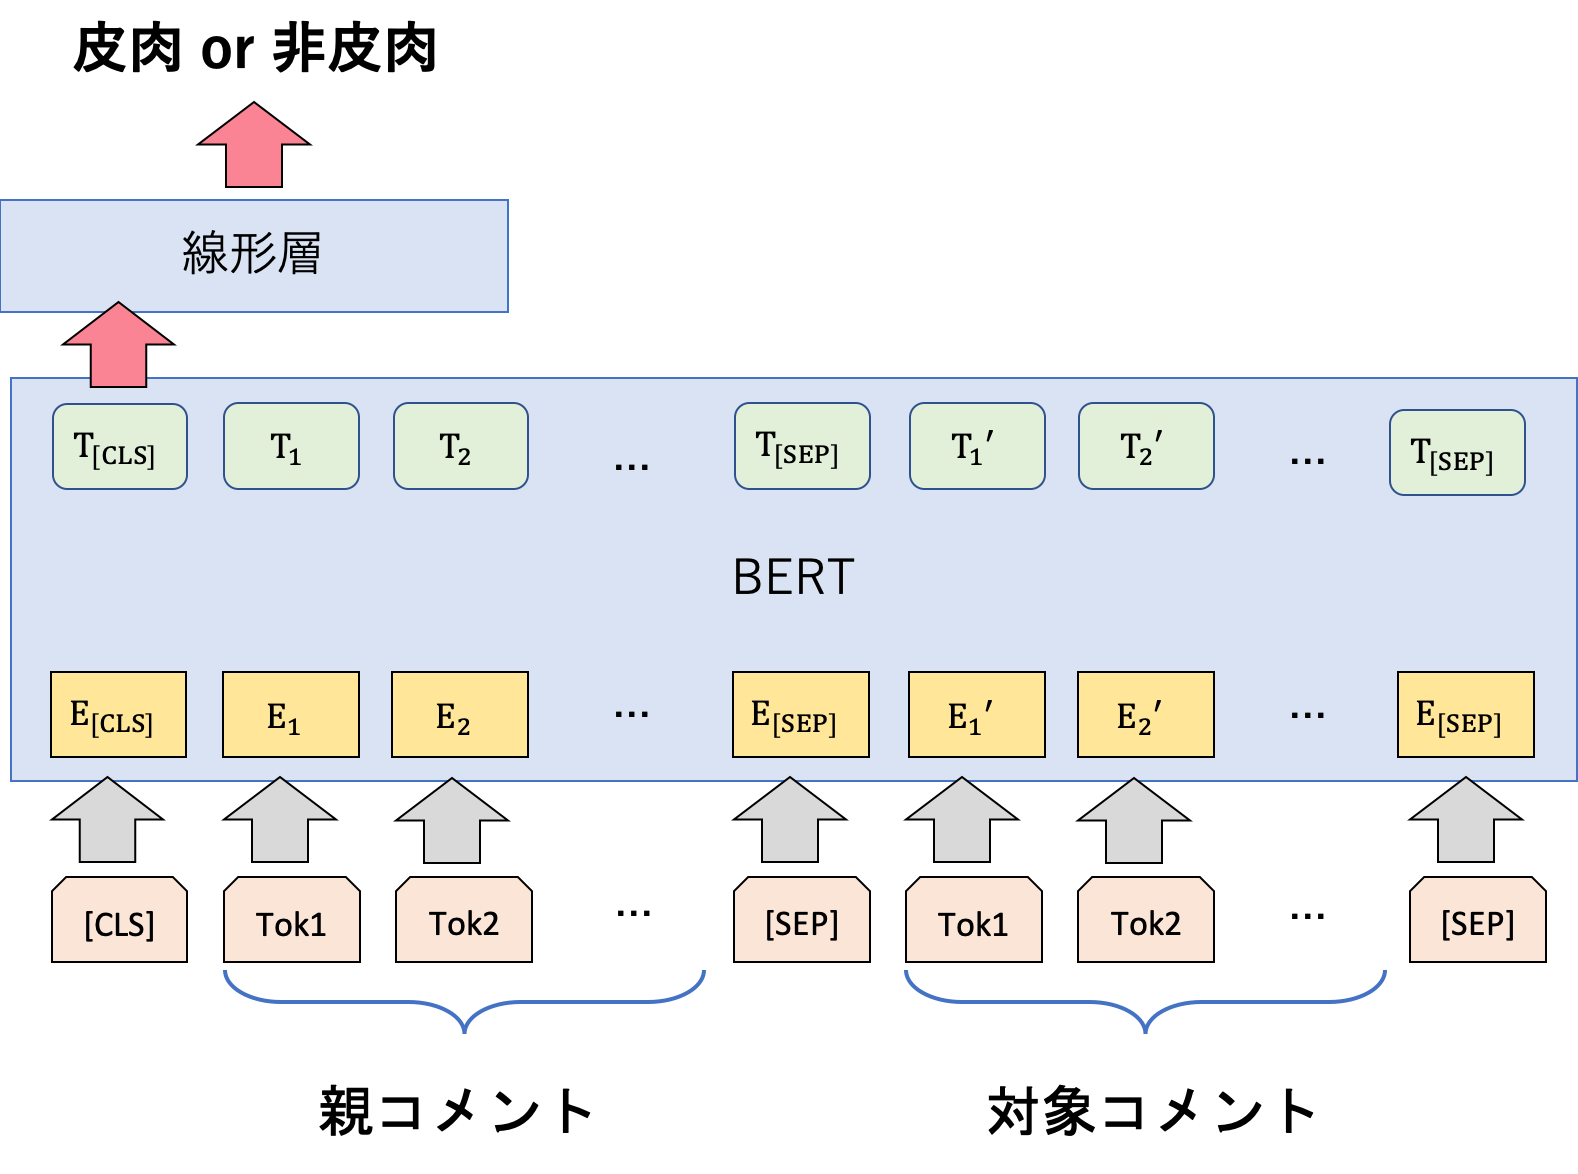
\includegraphics[width=0.8\linewidth]{./figure/40_model.png}
	 \end{center}
 \caption{実験モデルの概要}
 \label{fig:40_model}
 \end{figure}
% end figure


表 \ref{tb:4_bert_param} に実験のパラメータを示す.
BERT と線形層の学習率は予備実験によって値の範囲を定め,Optuna \cite{akiba2019optuna} によって探索した.
学習時は BERT の全層をファインチューニングし,線形層も重みを更新した.
\par

%%% table
\begin{table}[tb]
  \caption{実験パラメータ}
  \label{tb:4_bert_param}
  \centering
  \begin{tabular}{c c} \hline

\multicolumn{2}{c}{BERT} \\ \hline
モデル & bert-base-uncased \\ 
入力層次元数 & 512 \\
出力層次元数 & 768 \\
学習率 & $1 \times 10^{-6}$ 〜 $1 \times 10^{-4}$ \\ \hline
\multicolumn{2}{c}{線形層} \\ \hline
入力層次元数 & 768 \\
出力層次元数 & 2 \\
学習率 & $1 \times 10^{-6}$ 〜 $1 \times 10^{-4}$ \\ \hline
\multicolumn{2}{c}{学習} \\ \hline
エポック数 & 20 \\
バッチサイズ & 16 \\
損失関数 & Cross Entropy Loss \\
最適化関数 & Adam \\
 & $\left( 
 \begin{tabular}{c}
 \footnotesize{learning rate = 0.001} \\ \footnotesize{$\beta_1 = 0.9$, $\beta_2 = 0.999$}
 \end{tabular}
  \right)$ 
%最適化関数 & 
%	\begin{tabular}{c}
%	Adam \\ learning rate $= 0.001$ \\ $\beta_1 = 0.9$, $\beta_2 = 0.999$
%	\end{tabular}

\\ \hline
  \end{tabular}
\end{table}
% end



%%%%%%%%%%%%%%%%%%%%%%%%%%%%%%
\afterpage{\clearpage}
\subsection{実験 1 結果}
表 \ref{tb:4_bert_result} に実験結果を示す.
太字の項目はベースラインである random データセットでの評価値を上回ったことを表している.

%%% table
\begin{table}[tb]
  \caption{実験結果}
  \label{tb:4_bert_result}
  \centering
  \begin{tabular}{c c c c c} \hline

dataset & Accuracy & Precision & Recall & F1 score  \\ \hline
politics & \textbf{0.730} & \textbf{0.722} & \textbf{0.748} & \textbf{0.735} \\
AskReddit & 0.619 & 0.630 & 0.580 & 0.604 \\
worldnews & \textbf{0.690} & 0.655 & \textbf{0.803} & \textbf{0.721} \\
pcmasterrace & 0.648 & 0.635 & \textbf{0.698}  & \textbf{0.665} \\ \hline
random & 0.653 & 0.664 & 0.618 & 0.640 \\ \hline

  \end{tabular}
\end{table}
% end


表より random データセットでの評価値を上回った項目が多いことが分かる.
このことは,subreddit ごとに皮肉推定をすることが,推定精度向上に有効に働いていると考えられる.
また politics データセットでは全ての評価指標で random データセットでの皮肉推定精度を上回った.
一方で AskReddit データセットでは全ての評価指標で random データセットでの皮肉推定精度を下回った.
このことから,politics データセットの皮肉表現の特徴を上手く捉えることができ,正しく推定できていると考えられる.
反対に,AskReddit データセットは何らかの理由で皮肉推定が困難であったと考えられる.
その理由としては以下のことが考えられる.
\begin{itemize}
	\setlength{\itemsep}{-1mm}
\item 皮肉文章と非皮肉文章が類似している
\item 皮肉・非皮肉ラベル付けが適切でない
\item 訓練データとテストデータの違いが大きい
\end{itemize}

また worldnews データセットでは Recall の値が高くなった.
このことは,データセットに含まれる皮肉データに対して皮肉であると正しく予測したものが多いことを表している.
反対に,Precision の値は random データセットでの評価値を下回り,このことは,皮肉であると予測したデータのうち真のラベルが皮肉であったものが少なかったことを表している.
すなわち,真のラベルが非皮肉であるものに対して皮肉であると予測したものが多いことを意味している.


%%%%%%%%%%%%%%%%%%%%%%%%%%%%%%
\afterpage{\clearpage}
\subsection{実験 2}

次に,politics,AskReddit,worldnews,pcmasterrace のデータセットに対して,学習時とテスト時で異なるデータセットを使用して皮肉推定をした.
実験の手順は実験 1 と同様である.


%%%%%%%%%%%%%%%%%%%%%%%%%%%%%%
\afterpage{\clearpage}
\subsection{実験 2 結果}
表 \ref{tb:4_result2} に実験結果を示す.
各項目の数値は Accuracy の値である.


%%% table
\begin{table}[b]
  \caption{実験結果}
  \label{tb:4_result2}
  \centering
  \begin{tabular}{c c c c c} \hline

\multirow{2}{*}{テストデータ} & \multicolumn{4}{c}{訓練データ} \\ \cline{2-5}
 & politics & AskReddit & worldnews & pcmasterrace \\ \hline
politics & \underline{0.730} & 0.640 & 0.690 & 0.637 \\
AskReddit & 0.586 & \underline{0.619} & 0.591 & 0.591 \\
worldnews & 0.723 & 0.652 & \underline{0.690} & 0.646 \\
pcmasterrace & 0.613 & 0.583 & 0.598 & \underline{0.648} \\ \hline

  \end{tabular}
\end{table}
% end



この結果について,各データが 5 つのモデルのうちいくつで正解したかを調べた.
表 \ref{tb:4_result3} に結果を示す.
各項目の数値はデータ数である.
なお正解したモデルの数が 0 とは,5 つ全てのモデルで誤識別したことを表している.

%%% table
\begin{table}[tb]
  \caption{正解したモデルの数とラベルの内訳}
  \label{tb:4_result3}
  \centering
  \begin{tabular}{c c c c c c c c} \hline

\multirow{2}{*}{ラベル} & \multicolumn{6}{c}{正解したモデルの数} & \multirow{2}{*}{合計} \\ \cline{2-7}
 & 5 & 4 & 3 & 2 & 1 & 0 & \\ \hline
皮肉 & 2255 & 1220 & 966 & 906 & 905 & 713 & 6965 \\
非皮肉 & 2087 & 1722 & 1206 & 792 & 610 & 548 & 6965 \\ \hline
合計 & 4,342 & 2942 & 2172 & 1698 & 1515 & 1261 & 13930 \\ \hline

  \end{tabular}
\end{table}
% end


次に,5 つ全てのモデルで誤識別したデータの内訳を調べた.
表 \ref{tb:4_result4} に統計を示す.
各項目の数値はデータ数で,括弧内は各データセットの各ラベルのデータ数における割合である.
例えば AskReddit データセットに含まれる皮肉データは 1503 件であり,そのうち全てのモデルで誤識別したデータは 260 件で 17.3\% にあたる.

%%% table
\begin{table}[tb]
  \caption{全てのモデルで誤識別したデータの内訳}
  \label{tb:4_result4}
  \centering
  \begin{tabular}{c c c c c} \hline

\multirow{2}{*}{データの所属データセット} & \multicolumn{4}{c}{ラベル} \\ \cline{2-5}
 & \multicolumn{2}{c}{皮肉} & \multicolumn{2}{c}{非皮肉} \\ \hline
politics & 102 & (6.0\%) & 160 & (9.4\%) \\
AskReddit & 260 & (17.3\%) & 82 & (5.5\%) \\
worldnews & 56 & (5.0\%) & 115 & (10.2\%) \\
pcmasterrace &107 & (12.1\%) & 60 & (6.8\%) \\
random & 188 & (10.7\%) & 131 & (7.5\%) \\ \hline

  \end{tabular}
\end{table}
% end





%%%%%%%%%%%%%%%%%%%%%%%%%%%%%%
\afterpage{\clearpage}
\subsection{考察}

\subsection{t-SNE を用いた次元圧縮による可視化}
図 \ref{fig:40_tsne1} 〜 図 \ref{fig:40_tsne5} に t-SNE によって次元圧縮し可視化した結果を示す.
各データセットの訓練データによりファインチューニングした BERT にテストデータを入力し,出力として得られる分散表現のうち [CLS] の分散表現を次元圧縮した.
各図の (a) は橙色が皮肉データを,青色が非皮肉データを表している.(b) は灰色が皮肉・非皮肉を正しく識別したデータを,黒色が誤って識別したデータを表している.
各図 (a) より,皮肉データと非皮肉データの分布に大きな差はないことから,BERT が皮肉表現の特徴を学習できたために皮肉推定が可能となったと考えられる.
また各図 (b) より,皮肉データと非皮肉データが混在している箇所の皮肉推定を誤っており,その範囲は全体にわたっていることが分かる.
このことから,皮肉表現は多様であり,一律の基準による皮肉推定は適切ではないと考えられる.


%%% figure minipage
\begin{figure}[b]
\begin{center}
 	\begin{minipage}{0.4\hsize}
	\begin{center}
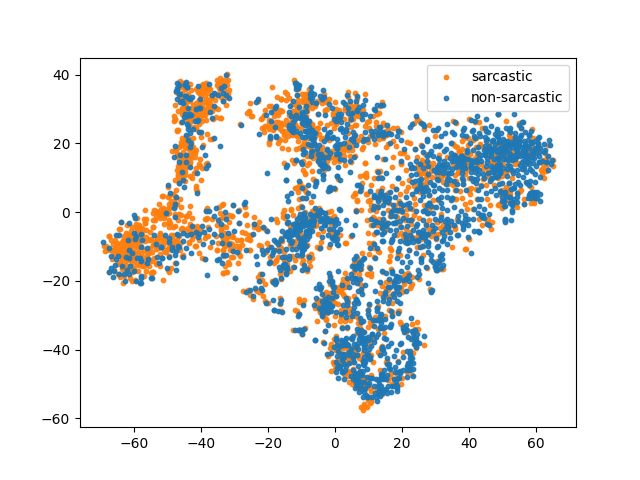
\includegraphics[width=\linewidth]{./figure/tsne_sarc_pol.png}
		 \subcaption{皮肉・非皮肉}
	\end{center}
%		\label{fig:40_tsne1-1}
	\end{minipage}
 	\begin{minipage}{0.4\hsize}
	\begin{center}
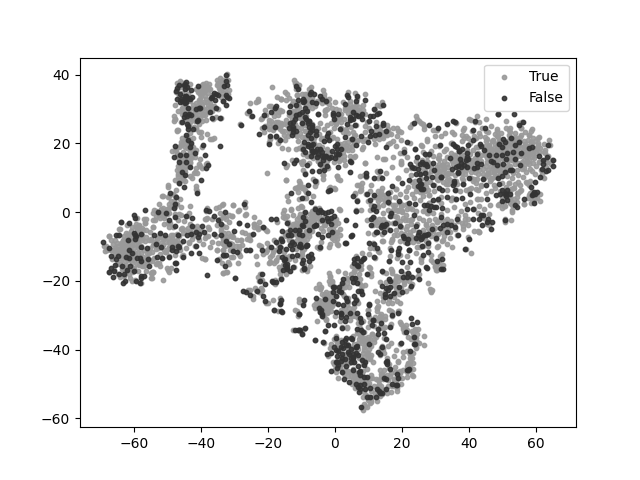
\includegraphics[width=\linewidth]{./figure/tsne_TorF_pol.png}
		\subcaption{正解・不正解}
 	 \end{center}
%		\label{fig:40_tsne1-2}
 	\end{minipage}
	\caption{t-SNE による可視化 (politics)}
	\label{fig:40_tsne1}
\end{center}
\end{figure}
% end figure

%%% figure minipage
\begin{figure}[tb]
\begin{center}
 	\begin{minipage}{0.4\hsize}
	\begin{center}
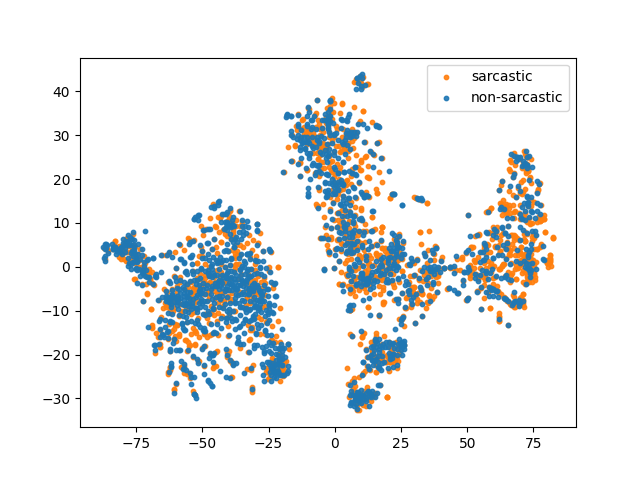
\includegraphics[width=\linewidth]{./figure/tsne_sarc_ask.png}
		 \subcaption{皮肉・非皮肉}
	\end{center}
%		\label{fig:40_tsne2-1}
	\end{minipage}
 	\begin{minipage}{0.4\hsize}
	\begin{center}
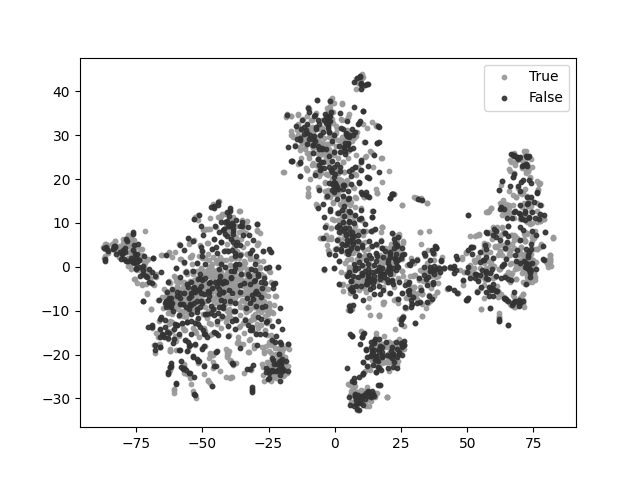
\includegraphics[width=\linewidth]{./figure/tsne_TorF_ask.png}
		\subcaption{正解・不正解}
 	 \end{center}
%		\label{fig:40_tsne2-2}
 	\end{minipage}
	\caption{t-SNE による可視化 (AskReddit)}
	\label{fig:40_tsne2}
\end{center}
\end{figure}
% end figure

%%% figure minipage
\begin{figure}[tb]
\begin{center}
 	\begin{minipage}{0.4\hsize}
	\begin{center}
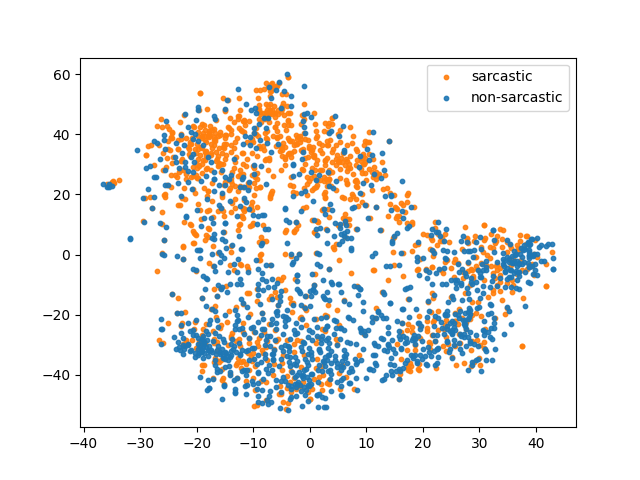
\includegraphics[width=\linewidth]{./figure/tsne_sarc_world.png}
		 \subcaption{皮肉・非皮肉}
	\end{center}
%		\label{fig:40_tsne3-1}
	\end{minipage}
 	\begin{minipage}{0.4\hsize}
	\begin{center}
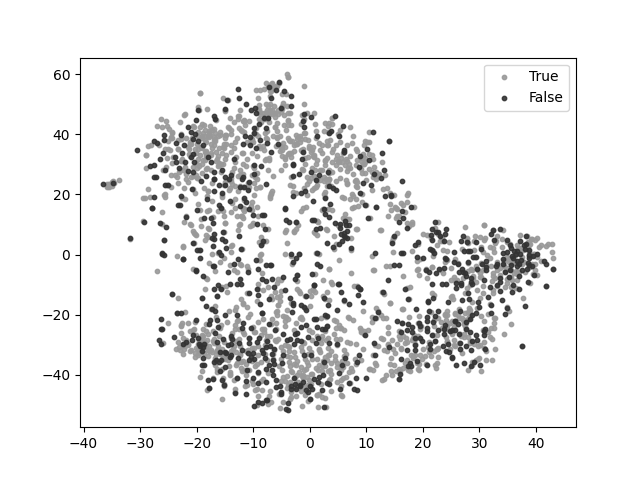
\includegraphics[width=\linewidth]{./figure/tsne_TorF_world.png}
		\subcaption{正解・不正解}
 	 \end{center}
%		\label{fig:40_tsne3-2}
 	\end{minipage}
	\caption{t-SNE による可視化 (worldnews)}
	\label{fig:40_tsne3}
\end{center}
\end{figure}
% end figure

%%% figure minipage
\begin{figure}[tb]
\begin{center}
 	\begin{minipage}{0.4\hsize}
	\begin{center}
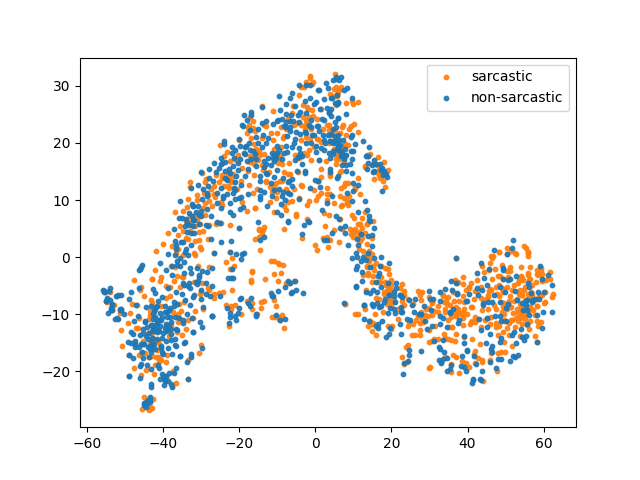
\includegraphics[width=\linewidth]{./figure/tsne_sarc_pc.png}
		 \subcaption{皮肉・非皮肉}
	\end{center}
%		\label{fig:40_tsne4-1}
	\end{minipage}
 	\begin{minipage}{0.4\hsize}
	\begin{center}
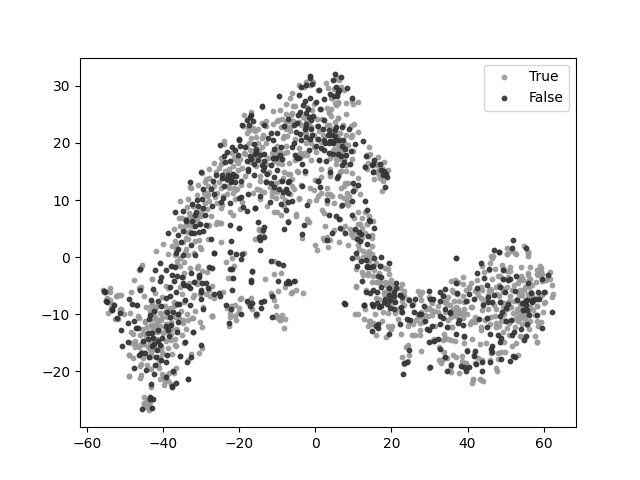
\includegraphics[width=\linewidth]{./figure/tsne_TorF_pc.png}
		\subcaption{正解・不正解}
 	 \end{center}
%		\label{fig:40_tsne4-2}
 	\end{minipage}
	\caption{t-SNE による可視化 (pcmasterrace)}
	\label{fig:40_tsne4}
\end{center}
\end{figure}
% end figure

%%% figure minipage
\begin{figure}[tb]
\begin{center}
 	\begin{minipage}{0.4\hsize}
	\begin{center}
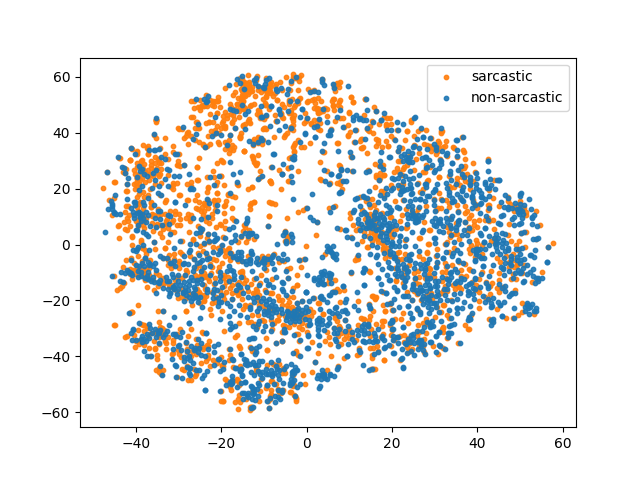
\includegraphics[width=\linewidth]{./figure/tsne_sarc_random.png}
		 \subcaption{皮肉・非皮肉}
	\end{center}
%		\label{fig:40_tsne4-1}
	\end{minipage}
 	\begin{minipage}{0.4\hsize}
	\begin{center}
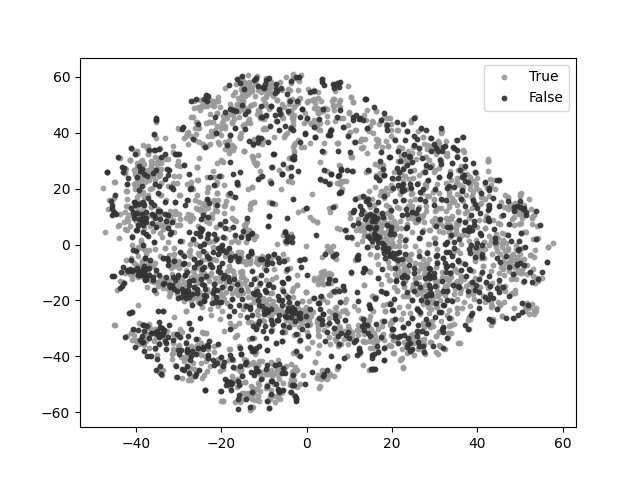
\includegraphics[width=\linewidth]{./figure/tsne_TorF_random.png}
		\subcaption{正解・不正解}
 	 \end{center}
%		\label{fig:40_tsne4-2}
 	\end{minipage}
	\caption{t-SNE による可視化 (random)}
	\label{fig:40_tsne5}
\end{center}
\end{figure}
% end figure




%%%%%%%%%%%%%%%%%%%%%%%%%%%%%%

%\subsubsection{GlobalOffensive,AskReddit で精度が低下したことへの考察}
%
%まず,各データセットの中身を見てみる.
%
%\begin{enumerate}
%\item[例 1] aaa
%\item[例 2] bbb
%\end{enumerate}




